\section{Results}
\label{sec:results}

The primary experiment is the Class~A search for a drifting, unresolved
carrier: \NWinA{} fine-channel windows toward \NSysClassA{} systems,
\EdrNWinA{} of them channelised finely enough to tell a drifting carrier from
a stationary one (\S\ref{sec:statistic}). The secondary Class~B search, for an
unresolved spectral excess with no drift discrimination, uses \NWinB{} coarse
windows. Together they are the \NWindows{} windows of the primary census.

\subsection{Sensitivity: the power at which a carrier would have crossed
the threshold} \label{sec:pninetysel}

\emph{The median system, on its best window, would have produced a threshold
crossing from a carrier of $\EirpNinetySysMedA$\,W.} Across the \NSysALim{}
systems with a constrained window the limits run from $\EirpNinetySysLoA$ to
$\EirpNinetySysHiA$\,W (Fig.~\ref{fig:classasens}); \NSysEfifteen{} of them
reach $10^{15}$\,W, and the median Class~A \emph{window} reaches
$\EirpNinetyWinMedA$\,W. Each limit is taken over the channels the line mask
leaves in the star's own rest frame (\S\ref{sec:summary}). The finest windows
were tuned to CO: a \UmFineChanKHz\,kHz window spans \UmFineBwMHz\,MHz against
a mask \UmFineMaskMHz\,MHz wide, so \UmNWinAFull{} of the \NWinA{} Class~A
windows lie wholly inside it and constrain nothing, and \NSysALostName{} has no
limit. Restricted to the \EdrNWinA{} drift-resolving windows
(\EdrUnionGHz\,GHz toward \EdrNSys{} systems), a system's limit is a median
\ScEdrMedPct{} per cent \ScEdrMedSense. In
\FcNBlock{} blocks whose in-beam fields were recombined after the limits were
computed, the search ran on the recombined data, so the limits of the
\FcNSys{} systems such a block sets are conservative, by a median factor
\FcMedFactor{} and at most \FcMaxFactor.

Carriers were injected at a random sub-channel phase and a random drift from
each window's own grid, and recovered through the unchanged pipeline to the
localisation at the star. Nine in ten come back at
$\EirpNinetyMultA\,P_{\rm trig}$ in Class~A, $P_{\rm trig}$ being the bare
$\LtCommonSnr\sigma$ of the window itself, and that power is
$\mathrm{EIRP}_{90}$. It does not depend on the brightness of the control ring
(Fig.~\ref{fig:strata}), and the correlator's spectral response is carried by
the injected tones (Appendix~\ref{app:conventions}). The \NCtrl-position
spatial rank is not charged against it: that would cost a further factor
$\SensCostLike$, and in \SensNRingHiUnres{} bright-ring windows it could not be
met at any injected power. Class~B carries its own factor,
$\EirpNinetyMultB\,P_{\rm trig}$, from \SensNToneCoarse{} carriers injected
into \SensNInjCoarse{} coarse windows. The calibration interval of the class factor,
$\times\SensFacLo$--$\times\SensFacHi$ (Table~\ref{tab:p90budget}), applies to the median and the counts and not to any one window. It places the
median system at $\TfMedCalLo$ to $\TfMedCalHi$\,W, so the second figure of that
median is set by the calibration and not by the depth of any observation.

\emph{Carriers were injected directly into \SensNInj{} of the \NWinA{}
Class~A windows, \SensNInjPct{} per cent, and the result transferred to the
other \SensNTransfer; that transfer is the dominant caveat on these limits.}
The injected windows, whole execution blocks drawn at random and balanced by
band and array, match the population in the median to \RpCovOtherPct{} per
cent on five of \RpNAxis{} properties and differ by $\times\RpCovWorstRatio$
on the sixth, \RpCovWorstAxis{} (Appendix~\ref{app:persys}). Only the ninety
per cent point in units of each window's own trigger power is carried across.
Over the injected windows that point ranges from $\times\SensIndivFacLo$ to
$\times\SensIndivFacHi$ of the adopted factor, \NmDispNTenth{} of the
\SensNInj{} lying within a tenth of it, and \emph{that dispersion, not the
calibration interval, is what one uninjected window's limit is uncertain by}.
On the five properties that set the reading, \NgNInterpWin{} of the
\SensNTransfer{} transferred windows lie inside the injected range on every
one and \NgNExtrapWin{} outside it on at least one, where that range is not an
empirical bound. \NgExtrapTakeClause{}, and none is among the \NSysEfifteen{}
systems reaching $10^{15}$\,W. The best window was itself injected into for
\SmcNMeasSys{} of the \NSysALim{} systems, marked in Table~\ref{tab:persys};
for the other \SmcNEstSys{} the headline limit is an estimate carrying that
dispersion, so \emph{the median is a calibration-transferred estimate and not
a measured sensitivity}. Drawing each transferred window's factor from the
\SensNInj{} measured ones, once per execution block over \SvNTrial{} trials,
lowers the median by \SvRsMedShiftPct{} per cent and leaves
\SvRsBlkNLo--\SvRsBlkNHi{} systems at $10^{15}$\,W in nine trials in ten.
Only \SvUncInNames{} can be moved across that level by the calibration
interval, the spread or the decorrelation\SvUncOutClause; each system's
probability is in the data archive.

\emph{Every limit is nominal in one respect: it excludes atmospheric
decorrelation}, which an injected carrier does not suffer and a real one does.
Estimated from each block's phase-calibrator phase rms
\citep[\S\S10.4.11, 11.3.1]{ALMAHandbook} with the phase-scatter relation of
\citet[Eq.~3]{Richards2022}, it leaves the median system's best window optimistic by \NmDecSysMedPct{} per
cent; it exceeds a tenth for \NmDecNBigSys{} systems and reaches
\NmDecSysWorstPct{} per cent for \NmDecSysWorstName. Divided out, it moves the median limit by
\NmDecAdjShiftPct{} per cent and takes the \NSysEfifteen{} systems reaching
$10^{15}$\,W to \NmDecAdjNEfifteen. It is stated and not applied because only \SensDecorNBlk{} of
\SensDecorNBlkTot{} blocks record the phase rms; the rest, estimated from
blocks matched in baseline, are measurably the harder ones.
Table~\ref{tab:persys} gives it system by system and the adjusted limits are
in the data archive. The spectral response biases the other way. The
injected tones fall \InjShortPct{} per cent short of the exact channel response
of a window without online spectral averaging. For the \SvNWinNAvg{}
Class~A windows delivered with averaging the exact factor is
$\SvRespFacTwo\,P_{\rm trig}$ (two-channel averaging, \SvNWinNTwo{} of them)
rather than $\EirpNinetyMultA\,P_{\rm trig}$, so their limits are conservative
and would fall to $\times\SvRespRatioTwo$ (Appendix~\ref{app:conventions}).
That is stated and not applied, because no carrier was injected through the
averaged response; an injection campaign using it is the remedy. \emph{The net
bias on one limit is therefore of either sign}: conservative by
\SvNetConsPct{} per cent in the median Class~A window, optimistic by
\SvNetOptPct{} per cent at the ninetieth percentile of the systems' best
windows.

\emph{A carrier that is not always radiating is penalised in proportion}: in
\DutyNTrial{} undrifted trials down to a \DutyCycleMinPct{} per cent duty cycle
the recovered amplitude followed it to \DutyAttenDevPct{} per cent, so a
transmitter on a tenth of the time needs $\DutyPowFac\times$ the power quoted;
the drifting intermittent case is unmeasured.

\begin{table*}
\centering
\scriptsize
\caption{What sets $\mathrm{EIRP}_{90}$, and in which direction. The
calibration interval applies to the class-average factor and so to any
statistic over many windows; the spread between windows is an observed
dispersion and is the statement about one window; the signed terms are biases
and are not folded into an error bar (\S\ref{sec:pninetysel}).}
\label{tab:p90budget}
\setlength{\tabcolsep}{2pt}
% GENERATED by sens_r11.py -- do not hand-edit.
\begin{tabular}{@{}l@{~~}r@{~~}>{\raggedright\arraybackslash}p{0.61\linewidth}@{}}
\hline
 & value & what it does to the limit \\
\hline
Class-average completeness & $\times3.03$ & nine carriers in ten recovered at this multiple of a window's own trigger power. \emph{Measured} in the 49 Class~A windows injected directly and \emph{estimated}, at this factor, in the other 356 \\
\hline
\multicolumn{3}{@{}l}{\emph{Uncertainty on that calibration} (per cent), combined in quadrature} \\
The factor itself & $\pm2$ & sampling error of the pooled value over the 49 injected windows \\
Absolute flux scale & $\pm\BudFlux$ & the observatory's own band-dependent specification (\BudFluxSource): \BudFluxSpec, weighted over this sample's bands \\
Distance and visibility scale & $\pm\BudDistVis$ & the Gaia parallaxes, which enter as $d^{2}$, and the block-to-block visibility scale \\
\emph{Combined} & $-11/+11$ & $\times0.89$--$\times1.11$ on the factor, and so on the median limit and on the system counts; $\pm\BudCombWorst$ for the \BudNHiWin{} Class~A windows in \BudHiBandWord~\BudHiBands, at \BudHiGHzList\,GHz \\
\hline
\multicolumn{3}{@{}l}{\emph{Spread between windows}. An observed dispersion, not an error bar.} \\
Window to window & $\times0.80$--$\times1.58$ & the 49 injected windows resolve 2.41--4.80\,$P_{\rm trig}$ individually, \NmDispNTenth{} of them within a tenth of the pooled value and the second largest at $\times\NmDispSecond$. This, and not the interval above, is what an estimated limit is uncertain by; it is wider, and it applies to \SmcNEstSys{} of the \NSysALim{} systems \\
\hline
\multicolumn{3}{@{}l}{\emph{Applied} window by window where a record allows it and bounded where none does, and so not combined with the above.} \\
Intra-integration smearing & $\times1.00$--$\times\SmcFacWorst$ & a carrier sweeps through part of a channel within one integration and the injected ones do not: $\eta_{\rm smear}$ at the drift that sets a ninety per cent point, from each window's own integration length where it is recorded (\SmcNMeas{} windows) and from the longest delivered anywhere where it is not (\SmcNBound) \\
Primary beam & $\times1.00$--$\times\NmBeamFacWorst$ & the star is not at the pointing centre, so each limit is divided by the response at its own offset, on the full width the observatory documents. Nothing in the median window; the \BmNAboveTenPct{} windows furthest off-axis carry the departure of that form from a blocked circular aperture, up to \BmModelMaxPct{} per cent, as a one-sided systematic \\
Annual parallax & $\times1.00$--$\times2.06$ & the phase centre omits it, so each limit is divided by the amplitude a compact source retains at its own displacement, a median \PxaLossMedPct\,per cent on the \PxaNWin{} windows carrying a parallax record; on the other \PxaNMissing{} the loss is bounded (Appendix~\ref{app:pbresp}) \\
\hline
\multicolumn{3}{@{}l}{\emph{Signed terms}. A bias is not an error bar and is not added to one.} \\
Channel response & $\times\RpRespFac$ & one over the share of a channel-confined carrier the peak channel keeps. Carried by the injections, so already inside the completeness above, which is this factor times a margin of $\times\RpMarginNinety$ over the nominal trigger \\
\quad its residual & $+\InjShortPct$, $+\SvRespShortPctTwo$ & the injected profile falls short of the exact response, without and with online spectral averaging ($N=1$, $N\geq2$; Appendix~\ref{app:conventions}): \emph{conservative} \\
Decorrelation & $+0/+\NmDecSysWorstPct$ & measured block by block from the phase rms the observatory records on each block's phase calibrator, which an injected carrier does not suffer and a real one does. One-sided, and a floor. A median $+\NmDecSysMedPct$ on the systems' best windows, $+\SensDecorHiPct$ above \SensDecorHiGHz\,GHz, and more than $+\SensDecorTailLevelPct$ in \SensDecorTailPct{} per cent of windows \\
\hline
\end{tabular}

\end{table*}

\begin{figure}
\centering
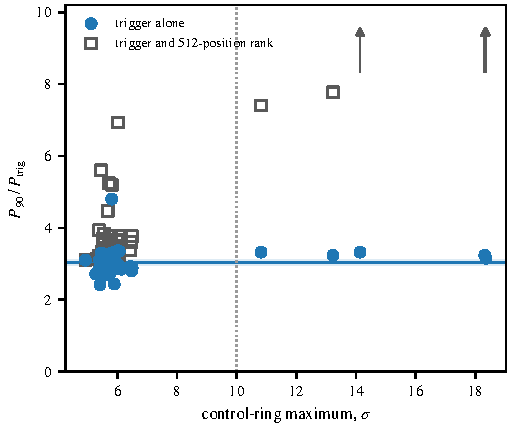
\includegraphics[width=\columnwidth]{figures/sens_ring.pdf}
%% ★ v4.26 (r25-captions): 9 printed lines -> R1 §7's limit of about six.
%% \S\ref{sec:pninetysel} above already carries every statement removed:
%% that the value does not depend on the ring's brightness, what charging
%% the rank would cost, and the bright-ring windows that cannot meet it at
%% any injected power -- the arrows.  \SensRingRule had this caption as its
%% only citation site, so the dotted line's threshold MOVED into that
%% paragraph rather than being dropped.
\caption{Why one completeness factor serves the whole class. The
\SensNInj{} directly injected Class~A windows at the power recovering nine
carriers in ten, each against its own \NCtrl-position ring maximum: no trend
with the ring. Filled, the criterion adopted here, pooled value as line and
band; open, the rank charged too, arrows where no power meets it; dotted, a
resolved ring.}
\label{fig:strata}
\end{figure}

\begin{figure}
\centering
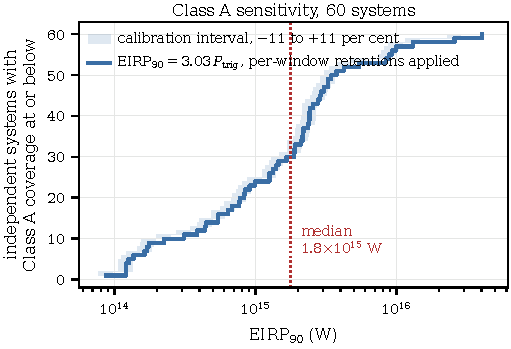
\includegraphics[width=\columnwidth]{figures/classa_sensitivity.pdf}
%% ★ r27 (R2-D10): panel (b), the Class A systems with a separated repeat
%% counted by system, duplicated Fig.~\ref{fig:confcov}b and LEAVES; Fig. 5
%% itself is protected and stays, one panel, one column.  Its four assertions
%% (\ZcConfSysDay, \ZcConfSysYr, \ZcNoRepSys, NSysClassA) still run in
%% make_fig_classa_sens.py.
\caption{\textbf{Single-epoch trigger completeness of the carrier search}:
the cumulative number of systems whose best window reaches a given
$\mathrm{EIRP}_{90}$, each window's own retentions applied and atmospheric
decorrelation excluded, the calibration interval of
Table~\ref{tab:p90budget} shaded. Confirmation needs a separated repeat,
which no power buys and which \ZcNoRepSys{} of the \NSysClassA{} systems lack
(Fig.~\ref{fig:waterfall}b; \S\ref{sec:mmdifferent}).}
\label{fig:classasens}
\end{figure}

\subsection{The nearest stars: Barnard's Star and Wolf~359}
\label{sec:barnardswolf}

Barnard's Star and Wolf~359 are the second- and third-nearest stellar systems
if brown dwarfs are excluded, and to our knowledge these are the first
millimetre or submillimetre technosignature limits for either; radio searches
of the nearest stars have worked at centimetre wavelengths
\citep{Enriquez2017,Price2020,Margot2023}. Both are non-detections, and
\emph{both limits come from the secondary Class~B search}, the archive holding
only coarse Band~6 windows toward them: Barnard's Star reaches
$\EirpNinetyBarnLo$--$\EirpNinetyBarnHi$\,W over \NWinBarn{} windows and
Wolf~359 $\EirpNinetyWolfLo$--$\EirpNinetyWolfHi$\,W over \NWinWolf.

\subsection{Threshold crossings and how each was disposed of}
\label{sec:technosearch}

Of the \NWindows{} windows of the primary census, \CsNCross{} hold a cell
reaching $T\geq5$ at the stellar position, all in data that pass the quality
criterion of Appendix~\ref{sec:blockquality}; the window flag of that appendix
reaches \DqNWin{} windows in \BkFlagNBlock{} blocks, and the
\BkFlagNCrossOther{} crossing it reaches, toward \BkFlagOtherStar, is withheld
from the amplitude-dependent tests. The $\pm\MaskHalfKms$\,km\,s$^{-1}$ line mask places \MkNCoinc{}
of the \CsNCrossQp{} within that velocity of a catalogued transition in the
star's own rest frame (Appendix~\ref{app:linemask}). Those \CsNAttrQp{} are attributed,
\LnAttrSupp{} with corroborating evidence of line emission and \LnAttrCoinc{}
on the coincidence alone, and \CsNUnattrQp{} are unattributed. The archival tail adds \CeNTailCrossWord{} more, both
unattributed and both toward \CeTailStar, in windows no expectation covers
(Table~\ref{tab:blockledger}); they are in the ledger and in none of the counts
above. The attributions are kinematic and not an accident of bandwidth: in
the correlator's frame the crossings crowd onto the transitions these setups
were tuned to (Appendix~\ref{app:rfi}). Of the \CsNCrossQp, \EvNLeadWord{} outrank all
\NCtrl{} control positions of their own window, \EvNRankQp{} of them
unattributed, and neither is present again at the cell its discovery predicts
(\S\ref{sec:vistest}). Behind each window's largest cell, \CkNSecondaryWord{}
weaker cells also reach the trigger; \CkNSecUnattrWord{} are unattributed and
\CkNRecurWord{} reaches the trigger in any covering block the recurrence test
reads. No crossing survives the chain, and this survey reports no detection; the
deposited crossing ledger lists every one.

\subsubsection{The unattributed count is what the control positions predict}
\label{sec:trigunif}

Because the searched channel\,$\times$\,drift cells per window span
\TuCellsDecades{} decades, the chance count is measured window by window over
the \CeNWin{} Class~A windows of the census, with one condition on both sides of
the comparison: a cell at the stellar position that reaches the trigger and
that the line mask does not attribute (Appendix~\ref{app:falsealarm}). These
fields' own control positions predict \CeExp{} unattributed Class~A crossings
and \CeObs{} are found. A count that large or larger arises by chance with
probability \CeProbNull{}, conditional on the control positions being a model
of the stellar position, the one assumption the searched data cannot test.
The expectation is not carried by a few noisy fields: without the
\BgTopNWord{} windows whose control positions trigger most often, the other
\BgDropTenNWin{} predict \BgDropTenExp{} against \BgDropTenObs{} observed. In \BgNConfIn{} of \BgNConf{} subsets by band, array, channel width and field
type the observed count lies within the central \CeCovPct{} per cent of its own
predicted distribution. Calibrated instead at the stellar-to-control ratio
\CeNear{} measured just below the trigger, the expectation is \CeExpNear{} at
$P=\CeProbNear$. A calibration error varying with frequency would raise the
star and not its continuum-free controls, but the least demanding window would
need \CyEpsMinPct{} per cent of its star's continuum to reach the trigger. The
excess below the trigger is not confined to windows with
the star within one synthesised beam of the phase centre, where an additive
visibility error would image (\BgPcOnRatio{} there, \BgPcOffRatio{} beyond). It appears only in the
7\,m-array data (\BgArrSevenRatio, against \BgArrTwelveRatio{} on the 12\,m
array), and its cause is not identified
(Appendix~\ref{app:radius}).

Both sides are read over the whole primary beam, the field of
\S\ref{sec:statistic}. The narrower field is the
extraction's original rule, which kept only the one entry whose phase centre
lies nearest the star and so drops on-source time and real signal; neither
rule has an adjustable radius. Read over that field on both sides, the same
comparison gives \FrNarrowObs{} against \FrNarrowExp{} at $P=\FrNarrowProb$.
Neither geometry was nominated as the primary before the counts were seen;
corrected for the \FrNRead{} readings the smaller probability is
\FrTwoTrialP, so neither departs from chance at the \CeAlphaPct{} per cent
level, a correction that assumes only these \FrNRead{} choices were made.
Neither reading establishes a population of non-astrophysical transmitters.
What the comparison could not have rejected is \CeAddLim{} further crossings
against these control positions (\FrNarrowAddLim{} on the narrower reading)
-- a count of
crossings, not of transmitting systems, and not an occurrence rate
(Appendix~\ref{app:falsealarm}).

\subsubsection{Stellar flares are excluded by a broadband prediction}

A millimetre flare raises every channel of a window alike. One able to
produce a single-channel crossing must therefore produce a $5\sqrt{N}\sigma$ continuum
event in the same integrations, \FlPredLo--\FlPredHi$\sigma$ for the windows
holding a crossing; the observed continuum statistic has a median of
\FlObsMed{} over the \FlNCont{} measurable crossings, with $|Z|<3$ in
\FlNQuiet. One block tests the case directly:
\FlEgStar{} \texttt{\FlEgEb} holds both a crossing ($T_\star=\FlEgT$) and the
millimetre flare of \citet{MacGregor2020}, which raises the continuum at
$Z=\FlEgContZ$ but contributes \FlEgContrib$\sigma$ to the single-channel
statistic, while the crossing's own de-drifted track reaches
$Z_{\max}=\FlEgTrackZ$.

\subsection{$\beta$~Pictoris: an astrophysical positive control, and the
obstacle it identifies} \label{sec:bpicval}

\emph{A search that finds nothing must show that it could have found
something.} The pipeline recovers the $\beta$~Pictoris circumstellar carbon
monoxide without being told the disc is there, in two rotational transitions
and \CsBpCoBlocks{} execution blocks spanning \BpBaselineYr\,yr, drawn from
\CsBpCoSess{} observing sessions. In the star's rest frame, at each block's own
epoch, all \BpicPanelNCo{} crossings lie within \BpicDvCoHi\,km\,s$^{-1}$ of the stellar
systemic velocity, in the two lowest CO transitions of a star with mapped
circumstellar CO \citep{Dent2014,Matra2017}. It is also the positive control of the recurrence test: every feature recurs
in another execution block, and each transition in another session.
In one block, \texttt{\BpCtrlBlock}, the resolved disc lifts the control ring
to \BpCtrlRingMax{} against \BpCtrlStar{} at the star
(Fig.~\ref{fig:bpiccontrol}): the rank tests compactness and not
authenticity, and extended emission shows instead in the \emph{level} of the
ring, on which the window flag of Appendix~\ref{sec:blockquality} is
defined.
HD~48370 is the complementary case, its crossing on the CO($2{\to}1$) that
\citet{Cataldi2023} report there and flag as possible cloud contamination
(Appendix~\ref{app:linemask}). The mask that removes such emission covers \FrNSpec{} species and costs
\MkMaskAPct{} per cent of the Class~A union bandwidth, and it is the single
most productive test in the chain (\S\ref{sec:mmdifferent}).

\subsection{The two crossings that lead their own control fields}
\label{sec:vistest}

Two crossings reach a stellar statistic above every one of the \NCtrl{}
control positions in their own window, and neither is a detection: \EvAStar{}
at \RqFreqSx\,GHz and \EvBStar{} at \RqFreqCp\,GHz, both in Band~\EvABand{}
and in the star's own rest frame (Table~\ref{tab:cand};
Fig.~\ref{fig:event}). Their rank says which crossing was examined first and
disposes of nothing (\S\ref{sec:summary}). Were the stellar and control
positions exchangeable, the control ensembles would predict \RkCondExp{} unattributed census crossings leading their field
by chance, and \RkCondNObsWord{} or more with probability \RkCondProb. Each
window contributes the share of its above-trigger controls that exceed every
other position, weighted as in Appendix~\ref{app:falsealarm}. In the reserved
blocks \RkHoLead{} of \RkHoN{} crossings lead their field, and beyond 40\,pc
\RkOosLead{} of \RkOosN.
\EvBStar's crossing lies $\EvBDv$\,km\,s$^{-1}$ from \EvBLine{} in the star's
frame, inside the mask, so it is \EvBDispo{} on that coincidence alone
(Appendix~\ref{app:linemask}). A visibility-domain fit, made for
\CsNVisFit{} of the \CsNCross{} census crossings and consistent with a point
source at the star for \CsNVisLocal, rejects neither: injected sources in the
bin these two occupy return ${\rm Re}/\sigma=\RsevReAtFiveMeanA\pm
\RsevReAtFiveSdA$.

Neither crossing is present when the same stellar-frame frequency is observed
again. The nearest covering block, \RcSxNearH{} and \EvBDeepH\,h from each
discovery, holds a line-like emitter returning to the predicted cell below
\RqNearFracSx{} and \RqNearFracCp{} of the discovery amplitude, and every
covering block combined, over \RqSpanDSx{} and \RqSpanDCp\,d, below
\RcSxFive{} and \RcCpFive. Each carrier's own fitted drift would leave that
half-channel cell ($\pm\RqDispSx$ and $\pm\RqDispCp$\,km\,s$^{-1}$) in
\ZtSxLeaveSec{} and \ZtCpLeaveSec\,s, so this is a line-recurrence check and
not a test of a drifting carrier (\S\ref{sec:etacrv}). At the faintest
amplitude consistent with each crossing having been found, the check would
have recovered such an emitter with calculated probability \RqPowerTrigSx{}
and \RqPowerTrigCp, and injected carriers measure \HjMeasSx{} and \HjMeasCp,
so for \EvBStar{} the silence does not exclude even a line-like emitter. In
Table~\ref{tab:cand}, $T_{\rm rep}$ is one cell at one trial and may be
negative, and the recovery chance in brackets, at the discovery amplitude, is
biased high. The
readings behind each bound are in
\texttt{candidates/repeat\_epoch\_readings.csv} of the data archive
\citep{SIdeposit}.

\subsection{Recurrence, applied across the unattributed crossings}
\label{sec:etacrv}

\emph{The widened window.} A transmitter in orbit changes its line-of-sight
velocity between epochs, so the broadest reading asks whether anything reaches
the trigger anywhere in a covering window, at any drift. That window is $\pm\WdHalfKms$\,km\,s$^{-1}$ wide in the median
case, wider than the $\pm\EcVexcKms$\,km\,s$^{-1}$ an orbit at the grid's
\WdAGrid\,m\,s$^{-2}$ ceiling can produce about any star here. \WuNWinExc{}
of the \WuNWin{} distinct covering windows hold a statistic above the
trigger, against the \WuExpWin{} chance predicts ($P=\WuProbWin$, or
\WuExpWinCtrl{} at $P=\WuProbWinCtrl$ when each window's own control positions
supply the rate; Appendix~\ref{app:falsealarm}). Every one of those windows
holds a crossing the ledger already lists, so the comparison re-reads the
trigger-level count of \S\ref{sec:trigunif} rather than adding a recurrence to it. \WuNWinExcTwo{} of the \WuNWinExc{} are
toward \WuTwoStars{}
(\S\ref{sec:twostars}); over the remaining \WuNWinRest{} windows the reading
is \WuNWinRestExc{} against \WuExpRest{} at $P=\WuProbRest$
(Appendix~\ref{sec:pairacct}).

\emph{The pair test.} Table~\ref{tab:pairs} asks of the \TjNPair{} pairs of
crossings inside that interval, across \TjNStarPair{} stars, whether one
transmitter could have produced both (Appendix~\ref{sec:pairacct}). Constant
line-of-sight acceleration requires equal drift rates, and the fitted rates
differ by more than the grid's resolution in \TjNUneqDrift{} of the
\TjNPair{} pairs, so the question becomes a weaker one: whether any trajectory inside the searched grid
joins the two. It separates
\TjNExcl{} of the \TjNPair{}; of the \TjNOpen{} it cannot separate, \TjNOpenPlain{}
are \emph{open} and \TjNPairEdge{} \emph{edge-limited}, and an open pair is not a
confirmation, since the comparison cannot accept an association
(\S\ref{sec:summary}). At each census window's own control rate chance puts
\OpExpSepRange{} open pairs in separated sessions
(\OpJoinPctLo--\OpJoinPctHi{} per cent of random pairs are joinable) against
the \OpObsSep{} observed, pairs with an archival-tail member set aside.

\emph{The predicted cell.} The \emph{line-recurrence check} reads the one cell
each discovery predicts at the repeat epoch, and so tests an emitter at rest in
the star's frame, as a line is, and not a carrier. The \RcNExcl{} bounded crossings accelerate at \ZtALosLo{} to
\ZtALosHi\,m\,s$^{-2}$ (\EgExStarALosLo{} to \EgStarALosHi{} in the star's
frame), which carries a carrier out of the half-channel in
\ZtLeaveSecLo{} to \ZtLeaveSecHi\,s (median \ZtLeaveSecMed); each crossing's nearest covering block is at
least \ZtGapOverLeaveMin{} times its own residence away. Carrying the fitted
drift forward does not rescue it: the drift's own resolution moves the
predicted cell by a median \ZtRegChanMed{} channels by the nearest repeat. On
lines the check works: \MkAttrRecur{} of the \MkAttrTested{} attributed
crossings tested recur in another session, \QcSepMinD--\QcSepMaxD\,d away,
and the \MkAttrExcl{} that do not are the faintest of them.
On the \RcNExclPoss{} unattributed crossings
whose cell could be read it returns nothing -- at most \RcTMatched{} at the
carried drift and \RcTMax{} at any drift, against a trigger of
\StageNullTrig. Over the \RcNExcl{} with a bound, a line-like emitter returning
to its cell is held to a median \RcFracMed{} of the discovery amplitude and
\RcFracMax{} at the weak end, where \HjNPowerLo{} are too shallow to test at the trigger amplitude. No bound
depends on the cell's registration, the anchor
or the threshold (Appendices~\ref{sec:nullscatter} and~\ref{sec:regbudget}).
\RcNoRepeatSentence No crossing is confirmed in the sense of
Table~\ref{tab:quantities}: none recurs at its predicted cell in a separated
session, and three separated crossings that one trajectory joins pairwise occur
toward \OpNTriAllWord{} star, \OpTriStars, counting archival-tail blocks, and
toward \OpNTriCenWord{} in the census alone.

\subsubsection{The reserved hold-out and the control beyond 40\,pc}
\label{sec:holdoutsearch}

Three sets of execution blocks enter no census statistic
(Table~\ref{tab:blockledger}); each was searched with the same pipeline. The \emph{hold-out}, \HoNBlock{} blocks,
\HoNWin{} windows, \HoNStar{} stars and \HoHours\,h on source set aside by the
identifier rule of Appendix~\ref{sec:heldout}, holds \HoNCross{} threshold
crossings, the strongest at $T_\star=\HoTMax$, none outranking its own control
positions. Of the \HoNTested{} tested for recurrence exactly one is present
again, a molecular line at $T_{\rm rep}=\HoRecTRep$; for the others the repeat
coverage holds a line-like emitter in the predicted cell to a median
\HoFracMed{} of the discovery amplitude and at most \HoFracMax. The
\emph{archival extension}'s \LdgExtWin{} windows in \LdgExtEB{} blocks hold
\QxObsCross{} crossings, \QxObsAttr{} inside the mask in their own star's frame
and \QxObsUnattr{} outside it, against \QxLam{} predicted by chance
(Appendix~\ref{app:falsealarm}). The probability of \QxObsUnattr{} or more is
\QxPGe, and the shortfall such a sample could have shown,
$P(0\,|\,\QxLam)=\QxPZero$, is not seen. The
\emph{control beyond 40\,pc}, \OosNBlock{} blocks and \OosNWin{} windows toward
\OosNStar{} stars (\OosHours\,h on source), holds \OosNCross{} crossings, the
strongest at $T_\star=\OosTMax$, none outranking its own controls. Read in the sky frame, it supports no limit and shows only that the pipeline behaves the
same way beyond the sample. The hold-out crossings are released row by row
with the crossing ledger.

%% Numbers are generated, not
%% typed: every \Tw... macro is written by twostars_r27.py (round 992), which
%% also writes tab_twostars_r27.tex.
\subsection{HD~14055 and \BkAlmaName}
\label{sec:twostars}

Of the \WuNWinExc{} covering windows above the trigger, \TwNWinExcTwoWord{}
are toward these two objects (Table~\ref{tab:twostars} lists every crossing
either holds). They are also the two most heavily observed objects in the
survey, holding \TwWinASharePct{} per cent of the Class~A census and
\TwNWinTwo{} of the \WuNWin{} covering windows, so \TwExpTwo{} of the
\WuExpWin{} expected exceedances are theirs before anything is looked at. HD~14055 holds \TwNExcHD{} against
\TwExpHD{} expected ($P=\TwProbHD$; its own control positions predict
\TwExpCtrlHD): its concentration is its exposure. \BkAlmaName{} holds
\TwNExcJx{} against \TwExpJx{} and \TwExpCtrlJx{} on the two nulls
($P=\TwProbJxRaw$ for this object alone). But it is the most discrepant of the
\TwLookNStar{} objects compared and was picked out for being so: chance puts
some object that far out in \TwLookPct{} per cent of realisations. It is a
target for follow-up, not evidence of a non-astrophysical source.

HD~14055's fields are ordinary: its control rings stand \TwRingQHD{} times
their class median, against \TwRingQSurv{} for the survey and \TwBlockQMax{}
for the rejected block. Its setups are continuum ones, and its crossings lie
\TwHDMaskLo--\TwHDMaskHi\,km\,s$^{-1}$ from the nearest masked transition in
its own frame. The \TwPairSpanD\,d baselines of Table~\ref{tab:pairs} come from its two
archival-tail crossings. The \TwHDNDeep{} epochs carrying the inverse variance
of those readings are follow-up blocks outside the census, and on them an
emitter at rest in the
stellar frame at the discovery amplitude (a line-like source) is excluded at
\TwHDExclA{} and \TwHDExclB$\sigma$; this does not test a drifting carrier
(\S\ref{sec:etacrv}).

\BkAlmaName{} is a serendipitous dwarf \TwPbJx{} arcsec off the phase centre
of fields pointed at the Lupus clouds, in \TwOnSrcJx\,s snapshots. Its
CO($2\to1$) crossing is cloud emission filling the field: it sits on a line
the observers tuned to, with a fitted drift \TwStepMin{} of a grid step from
zero and a control ring reaching $T_\star=\TwCtrlMaxJx$ against
\TwTStarCtrlJx{} at the star. The star has no measured systemic velocity, and
recomputing the attribution over $\pm\TwSweepHalfKms$\,km\,s$^{-1}$ changes
only that crossing, whose reading in the local standard of rest holds anyway
(Appendix~\ref{app:linemask}). What is left is
\TwNExcJxWord{} windows where \TwExpJx{} were expected, on
\TwJxNCrossExcWord{} crossings between \TwJxExcBandLo{} and
\TwJxExcBandHi\,GHz in \TwJxNBlockExcWord{} of this object's
\TwJxNBlockWord{} blocks. Their control rings are ordinary, their drifts far
from zero, and a visibility fit places \TwJxNLocalExcWord{} of the
\TwJxNCrossExcWord{} at the star. A transition of a wider \TwWideNSpecies-species list lies within
\TwWideDvMax\,km\,s$^{-1}$ of every crossing in Table~\ref{tab:twostars}, as
its \TwWideNTrans{} transitions guarantee, so a wider list identifies nothing.
We have no explanation. A repeat observation should point at \BkAlmaName,
with a radial velocity and one deeper epoch at
\TwJxExcBandLo--\TwJxExcBandHi\,GHz.

\begin{table}
\centering
\caption{\textbf{Every crossing toward HD~14055 and \BkAlmaName.} Rates are
in the observatory frame; $\ge$ and $\le$ mark a fit on the grid's outermost
trial.}
\label{tab:twostars}
\scriptsize
%% GENERATED by twostars_r27.py -- do not hand-edit.
\begin{tabular}{@{}r@{~}r@{~}r@{~}l@{~}r@{~}r@{}}
\hline
$\nu_\star$ & $T_\star$ & $\dot\nu_{\rm obs}$ & nearest masked & $\Delta v_\star$ & ${\rm Re}/\sigma$ \\
(GHz) & & (Hz\,s$^{-1}$) & transition & (km\,s$^{-1}$) & \\
\hline
\multicolumn{6}{@{}l}{\emph{HD~14055}} \\
331.254 & 5.10 & $+1635$ & $^{13}$CO($3$--$2$) & $+604$ & $+5.1$ \\
331.766 & 5.57 & $-3857$ & $^{13}$CO($3$--$2$) & $+1069$ & $+5.0$ \\
344.452 & 5.01 & $-2589$ & SO($8_{8}$--$7_{7}$) & $+123$ & -- \\
344.696 & 5.18 & $-2426$ & SO($8_{8}$--$7_{7}$) & $+336$ & $+4.8$ \\
345.092 & 5.17 & $+2123$ & SO($2_{3}$--$2_{1}$) & $-531$ & $+4.6$ \\
345.430 & 5.45 & $+2584$ & SO($2_{3}$--$2_{1}$) & $-238$ & -- \\
\hline
\multicolumn{6}{@{}l}{\emph{\BkAlmaName}} \\
216.204 & 5.25 & $-2198$ & SiO($5$--$4$) & $-1245$ & $-0.6$ \\
217.727 & 5.09 & $-983$ & H$_2$CO($3_{0,3}$--$2_{0,2}$) & $-680$ & $+1.8$ \\
218.669 & 5.05 & $-2023$ & H$_2$CO($3_{2,1}$--$2_{2,0}$) & $-125$ & $+4.5$ \\
218.892 & 5.11 & $+2373$ & H$_2$CO($3_{2,1}$--$2_{2,0}$) & $+181$ & $+4.7$ \\
230.539 & 5.39 & $-19$ & CO($2$--$1$) & $+2$ & $+4.4$ \\
347.189 & 5.01 & $-2581$ & SiO($8$--$7$) & $-122$ & $+4.6$ \\
\hline
\end{tabular}

\end{table}

\begin{figure*}
\centering
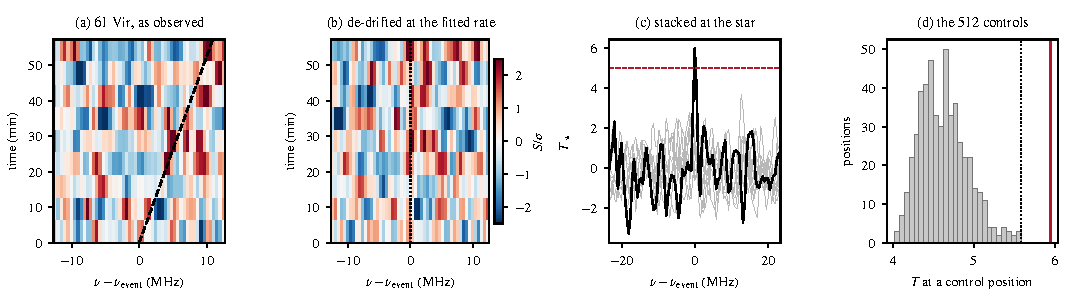
\includegraphics[width=\textwidth]{figures/event_crossings.pdf}
\caption{\textbf{The strongest unattributed crossing of the quality-passing
data, and the control field it leads.} Frequencies are in the star's rest
frame.
\emph{(a)}~The dynamic spectrum at \EvAStar's position around the crossing
at \RqFreqSx\,GHz, observed \EvADate, the fitted drift of
\EvADrift\,Hz\,s$^{-1}$ dashed, \EvANInt{} integrations binned into
\EvANBin{} and plotted in units of each bin's noise.
\emph{(b)}~The same rows shifted by that drift.
\emph{(c)}~The de-drifted stack at the star (black) and at the
\RcNRetCtrl{} control positions with retained dynamic spectra (grey), in
units of its own noise, the trigger dashed. \emph{(d)}~The same statistic at
each of the \NCtrl{} rank-screen control positions: the star (solid) against
the highest control (dotted).}
%% ★ v4.26 (r25-captions): 8 printed lines -> R1 §7's limit of about six.
%% MOVED into \S\ref{sec:vistest} above, carrying seven macros this caption
%% was the only citation site of (\EvAFlux, \EvAFluxErr, \EvARmsInt,
%% \EvAPerIntSig, \EvADwellMin, \EvADriftChan, \EvAChanwkHz,
%% \EvAElapsedMin): the per-integration significance and the drift's reach
%% across the block, both of which are statements about the crossing and not
%% keys to the panels.  DELETED: the closing pointer to
%% Table~\ref{tab:cand} and to \EvBStar{} at \RqFreqCp\,GHz, which
%% \S\ref{sec:vistest}'s own second paragraph states in the same words.
\label{fig:event}
\end{figure*}

\begin{table}
\centering
%% ★★★ v4.26 (r25-captions): 16 PRINTED LINES -> the author's limit.  Nothing
%% here was dropped on the floor: the $\pm\WdHalfKms$ interval and the
%% \TjNCandPair{} it holds are \S\ref{sec:etacrv}'s own second paragraph
%% already; \emph{edge} is defined there verbatim; and the subscript $\star$,
%% the observatory-frame pointer to Appendix~\ref{sec:edge} and the
%% \emph{Miss} column's units are now sentences in that same paragraph, which
%% is where a reader meets the table.  Measured with capmeasure.py.
\caption{\textbf{Can two crossings be one carrier?} The \TjNPair{} pairs
toward one star with an unattributed member (\S\ref{sec:etacrv}); the note
below defines the columns and the verdicts.}
\label{tab:pairs}
\scriptsize
%% GENERATED by pairs_v415.py -- do not hand-edit.
\begin{tabular}{@{}l@{~}l@{\,}c@{\,}r@{\,}r@{\,}r@{\,}r@{\hspace{3.5pt}}r@{~}l@{}}
\hline
Star & blocks & new & $\Delta t$ & $\dot\nu_{1\star}$ & $\dot\nu_{2\star}$ & $\Delta\nu$ & miss & one? \\
 & & sess. & (d) & \multicolumn{2}{c}{(Hz\,s$^{-1}$)} & (MHz) & grid & \\
\hline
61~Vir & X822/X82f & yes & 3.00 & $+1092$ & $+3221$ & $+755.4$ & 15 & open \\
J1537$-$3319 & X10359/X398 & yes & 123 & $-2000$ & $+2390$ & $+223.5$ & 3.6 & open \\
HD~14055 & X24be0/Xd46 & yes & 1.92 & $+1665$ & $-3823$ & $+512.7$ & 100 & open \\
 & X2b2ee/X3835 & yes & 2.09 & $-2390$ & $+2155$ & $+395.5$ & 55 & open \\
 & X3835/Xd526 & yes & 607 & $+2155$ & $-2563$ & $-640.4$ & -- & open \\
 & X2b2ee/Xd526 & yes & 609 & $-2390$ & $-2563$ & $-244.9$ & -- & open \\
 & X3835/X25c5e & yes & 649 & $+2155$ & $+2611$ & $+338.3$ & -- & open \\
 & X2b2ee/X25c5e & yes & 651 & $-2390$ & $+2611$ & $+733.8$ & -- & open \\
$\beta$~Pic & X3a90/Xa9df & no & 1.02 & $-1611$ & $-679$ & $+85.5$ & 132 & open \\
\hline
HD~285968 & X108f/X5b4e & yes & 4.99 & $-29$ & $-29$ & $-0.002$ & 0.6 & yes \\
 & X3bf6/X108f & yes & 39 & $-29$ & $-29$ & $-0.024$ & 0.6 & yes \\
 & X3bf6/X5b4e & yes & 44 & $-29$ & $-29$ & $-0.027$ & 0.6 & yes \\
\hline
\end{tabular}

\par\vspace{2pt}
{\scriptsize \emph{New sess.}: \emph{yes} where the two blocks belong to different
observing sessions. Starred rates are in the star's frame, the observatory's
own acceleration removed (observatory frame: Appendix~\ref{sec:edge}). \emph{Miss} measures
departure from constant acceleration, in units of the drift grid's resolution
over $\Delta t$; a dash marks a pair that resolution cannot separate. The
verdict is set by the bounded-trajectory test, which a constant-acceleration
failure does not decide -- a miss of \TjAcceptSig{} or less does, and sets
\emph{yes}; \emph{edge}, one rate lies on the grid's outermost trial and is
a lower bound. Below the rule, a control: the \TjCtlLine{} line of
\TjCtlStar, which does not drift.\par}
\end{table}

\begin{table}
\centering
%% ★★★ v4.26 (r25-captions): 15 PRINTED LINES -> the author's limit.  The row
%% stubs of tab_recurcand_v411 already label $T_{\rm pers}$, $T_{\rm rep}$,
%% $(T_{\rm rep}+5)/T_{\rm pers}$ and the $\Phi$ rows in words, so the caption
%% was re-stating the table.  What was NOT anywhere else -- the sign of
%% $T_{\rm rep}$ against the indented maxima, and "in brackets the same at $S$,
%% which is biased high" -- is now \S\ref{sec:vistest}'s prose, two
%% paragraphs above this float.  The half-channel displacement is already in
%% that section ($\pm\RqDispSx$, $\pm\RqDispCp$) and the pointer to
%% Fig.~\ref{fig:event} is already in its first paragraph.
\caption{\textbf{The two events}, the crossings whose
stellar statistic exceeds all \NCtrl{} control positions of their own window.
\S\ref{sec:vistest} reads them.}
\label{tab:cand}
\footnotesize
%% GENERATED by recur_v411.py -- do not hand-edit.
\begin{tabular}{@{}>{\raggedright\arraybackslash}p{0.49\columnwidth}@{~~}r@{~~}r@{}}
\hline
 & 61 Vir & CP$-$72 2713 \\
\hline
Frequency, stellar frame (GHz) & 346.323236 & 344.296455 \\
Drift rate (Hz\,s$^{-1}$) & $+3182$ & $-2056$ \\
$T_\star$ & 5.947 & 5.809 \\
Highest control $T$ & 5.58 & 5.68 \\
Fitted amplitude (mJy) & 118.6 $\pm$ 19.9 & 11.3 $\pm$ 2.0 \\
Peak-channel EIRP (W) & $5.0 \times 10^{14}$ & $8.9 \times 10^{14}$ \\
Repeat epochs measured & 3 & 5 \\
Nearest covering epoch, separation (h) & $-1.97$ & $+2.05$ \\
$T$ expected if persistent, $T_{\rm pers}$ & 9.69 & 6.29 \\
$T$ measured, matched drift, $T_{\rm rep}$ & $+0.36$ & $-0.88$ \\
Amplitude still bounded, $(T_{\rm rep}+5)/T_{\rm pers}$ & 0.55 $S$ & 0.65 $S$ \\
Calculated recovery chance $\Phi$ at $5S/T_\star$ (at $S$) & 1.00 (1.00) & 0.66 (0.90) \\
Nearest masked transition & SO($9_{8}$--$8_{7}$) & SO($8_{8}$--$7_{7}$) \\
\quad its offset $\Delta v_\star$ (km\,s$^{-1}$) & $-177.6$ & $-12.3$ \\
Disposition & not confirmed & attributed \\
\hline
\end{tabular}

\end{table}

%% ★★★★ TABLE 7 (tab:holdout) MOVED TO THE RELEASED FILES, round 25, to
%% the referees' guardrail "Table 7 may move to the catalogue".  It was a
%% full-width float of 0.20 pp carrying a 5-line full-width caption: 0.26 pp
%% in all, measured by floatinv.py and capmeasure.py.
%% ► ITS NAMED HOME, WHICH r25-zenodo MUST PROVIDE: the hold-out crossings as
%%   rows of the crossing ledger, carrying \Delta v_star (the offset from the
%%   nearest masked transition in the star's own frame), n_rep, T_pers, T_rep
%%   and the dagger flag for an offset inside the attribution interval whose
%%   species the attribution set excludes.  Sec. 5.6.2 carries the pointer.
%% ► NOTHING WAS DELETED FROM THE PROSE TO PAY FOR IT: the two readings the
%%   table carried that the text quoted, \HoRecTRep and \HoFracMax, are both
%%   still in Sec. 5.6.2; and the caveat its caption carried -- that a
%%   crossing inside the attribution interval whose species the set excludes
%%   is reported and not acted on -- is stated in Sec. 4.2 and Appendix C, so
%%   it survives exactly once, which is the referees' own rule.
%% ► To restore the float, revert this comment block; tab_holdout_v412.tex is
%%   still generated and still in make_all.sh.

%% tab:ledger MOVED to Appendix D (sections/app_J_falsealarm.tex): a
%% full-width 56-row table* worth 0.72 pp of the main text.  Sec. 5.3 and
%% Sec. 5.6 carry the counts and cite it.



%% fig:chain MOVED to sections/04_method.tex, Sec. 4.2, where it is first
%% cited (referee 2, minor 3).  Sec. 5 cites it at the crossing census.
